\newpage

\subsection{QuizziPedia::Front-End::ModelViews}
\subsubsection{Informazioni generali}
\label{QuizziPedia::Front-End::ModelViews}
\begin{figure}
	\centering
	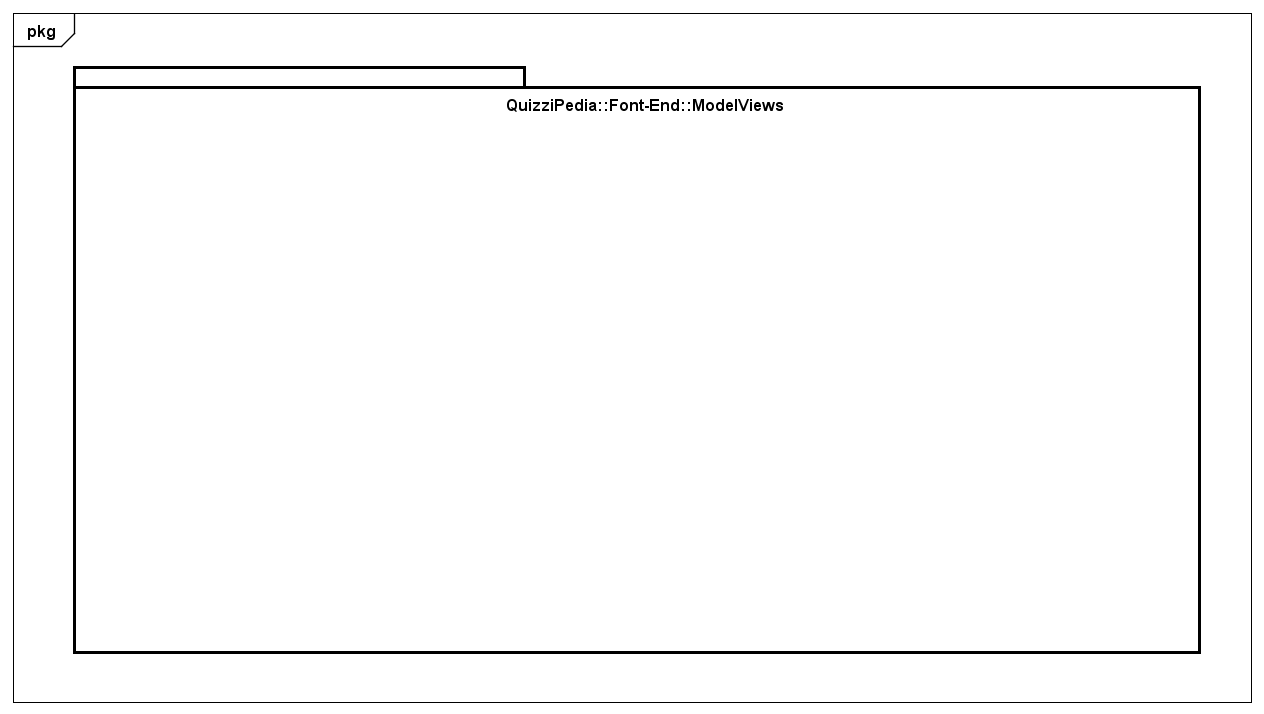
\includegraphics[scale=0.45]{UML/Package/QuizziPedia_Front-End_ModelViews.png}
	\caption{QuizziPedia::Front-End::ModelViews}
\end{figure}
\begin{itemize}
	\item \textbf{Descrizione}: package contenente le classi che saranno presenti nella variabile d'ambiente \texttt{\$scope} di \textit{Angular.js\ped{G}} che permettono il \textit{Two-Way Data-Binding\ped{G}} tra le views e i controllers;
	\item \textbf{Padre}: \texttt{Front-End};
	\item \textbf{Interazione con altri componenti}:
	\begin{itemize}
		\item \texttt{Controllers}: package contenente i controllers front-end dell'applicazione;
		\item \texttt{Directives}: package contenente le directives front-end dell'applicazione;
		\item \texttt{View}: package contenente le views front-end dell'applicazione;
		\item \texttt{Templates}: package contenente i templates necessari per la creazione dinamica delle viste per le domande.
	\end{itemize}
\end{itemize}
\subsubsection{Classi}
	
	\paragraph{QuizziPedia::Front-End::ModelViews::LoginModelView}
	
	\label{QuizziPedia::Front-End::ModelViews::LoginModelView}
	
	\begin{figure}[ht]
		\centering
		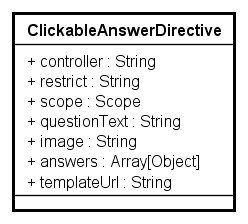
\includegraphics[scale=0.5,keepaspectratio]{UML/Classi/Front-End/QuizziPedia_Front-end_Templates_ClickableAnswerTemplate.png}
		\caption{QuizziPedia::Front-End::ModelViews::LoginModelView}
	\end{figure} \FloatBarrier
	
	\begin{itemize}
		\item \textbf{Descrizione}: ;
		\item \textbf{Utilizzo}: ;
		\item \textbf{Relazioni con altre classi}: 
		\begin{itemize}
			\item \textit{IN} \texttt{View}: ; 
			\item \textit{IN} \texttt{Controller}: ;
		\end{itemize}
		\item \textbf{Attributi}: 
		\begin{itemize}
			\item ;
		\end{itemize}
		\item \textbf{Metodi}: 
		\begin{itemize}
			\item ;
		\end{itemize}
	\end{itemize}
	
	\paragraph{QuizziPedia::Front-End::ModelViews::SignUpModelView}
	
	\label{QuizziPedia::Front-End::ModelViews::SignUpModelView}
	
	\begin{figure}[ht]
		\centering
		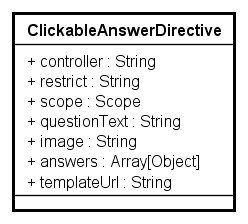
\includegraphics[scale=0.5,keepaspectratio]{UML/Classi/Front-End/QuizziPedia_Front-end_Templates_ClickableAnswerTemplate.png}
		\caption{QuizziPedia::Front-End::ModelViews::SignUpModelView}
	\end{figure} \FloatBarrier
	
	\begin{itemize}
		\item \textbf{Descrizione}: ;
		\item \textbf{Utilizzo}: ;
		\item \textbf{Relazioni con altre classi}: 
		\begin{itemize}
			\item \textit{IN} \texttt{View}: ; 
			\item \textit{IN} \texttt{Controller}: ;
		\end{itemize}
		\item \textbf{Attributi}: 
		\begin{itemize}
			\item ;
		\end{itemize}
		\item \textbf{Metodi}: 
		\begin{itemize}
			\item ;
		\end{itemize}
	\end{itemize}
	
	\paragraph{QuizziPedia::Front-End::ModelViews::PasswordForgotModelView}
	
	\label{QuizziPedia::Front-End::ModelViews::PasswordForgotModelView}
	
	\begin{figure}[ht]
		\centering
		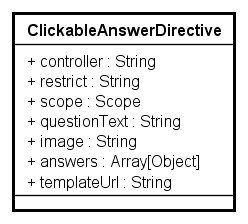
\includegraphics[scale=0.5,keepaspectratio]{UML/Classi/Front-End/QuizziPedia_Front-end_Templates_ClickableAnswerTemplate.png}
		\caption{QuizziPedia::Front-End::ModelViews::PasswordForgotModelView}
	\end{figure} \FloatBarrier
	
	\begin{itemize}
		\item \textbf{Descrizione}: ;
		\item \textbf{Utilizzo}: ;
		\item \textbf{Relazioni con altre classi}: 
		\begin{itemize}
			\item \textit{IN} \texttt{View}: ; 
			\item \textit{IN} \texttt{Controller}: ;
		\end{itemize}
		\item \textbf{Attributi}: 
		\begin{itemize}
			\item ;
		\end{itemize}
		\item \textbf{Metodi}: 
		\begin{itemize}
			\item ;
		\end{itemize}
	\end{itemize}
	
	\paragraph{QuizziPedia::Front-End::ModelViews::HomeModelView}
	
	\label{QuizziPedia::Front-End::ModelViews::HomeModelView}
	
	\begin{figure}[ht]
		\centering
		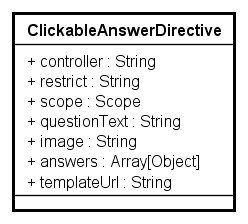
\includegraphics[scale=0.5,keepaspectratio]{UML/Classi/Front-End/QuizziPedia_Front-end_Templates_ClickableAnswerTemplate.png}
		\caption{QuizziPedia::Front-End::ModelViews::HomeModelView}
	\end{figure} \FloatBarrier
	
	\begin{itemize}
		\item \textbf{Descrizione}: ;
		\item \textbf{Utilizzo}: ;
		\item \textbf{Relazioni con altre classi}: 
		\begin{itemize}
			\item \textit{IN} \texttt{View}: ; 
			\item \textit{IN} \texttt{Controller}: ;
		\end{itemize}
		\item \textbf{Attributi}: 
		\begin{itemize}
			\item ;
		\end{itemize}
		\item \textbf{Metodi}: 
		\begin{itemize}
			\item ;
		\end{itemize}
	\end{itemize}
	
	\paragraph{QuizziPedia::Front-End::ModelViews::ResultsModelView}
	
	\label{QuizziPedia::Front-End::ModelViews::ResultsModelView}
	
	\begin{figure}[ht]
		\centering
		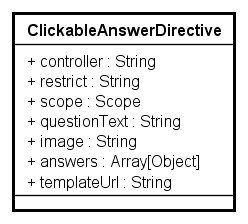
\includegraphics[scale=0.5,keepaspectratio]{UML/Classi/Front-End/QuizziPedia_Front-end_Templates_ClickableAnswerTemplate.png}
		\caption{QuizziPedia::Front-End::ModelViews::HomeModelView}
	\end{figure} \FloatBarrier
	
	\begin{itemize}
		\item \textbf{Descrizione}: ;
		\item \textbf{Utilizzo}: ;
		\item \textbf{Relazioni con altre classi}: 
		\begin{itemize}
			\item \textit{IN} \texttt{View}: ; 
			\item \textit{IN} \texttt{Controller}: ;
		\end{itemize}
		\item \textbf{Attributi}: 
		\begin{itemize}
			\item ;
		\end{itemize}
		\item \textbf{Metodi}: 
		\begin{itemize}
			\item ;
		\end{itemize}
	\end{itemize}
	
	\paragraph{QuizziPedia::Front-End::ModelViews::SearchQuestionnaireModelView}
	
	\label{QuizziPedia::Front-End::ModelViews::SearchQuestionnaireModelView}
	
	\begin{figure}[ht]
		\centering
		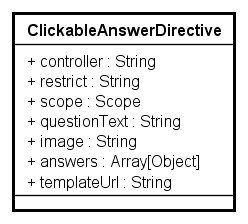
\includegraphics[scale=0.5,keepaspectratio]{UML/Classi/Front-End/QuizziPedia_Front-end_Templates_ClickableAnswerTemplate.png}
		\caption{QuizziPedia::Front-End::ModelViews::HomeModelView}
	\end{figure} \FloatBarrier
	
	\begin{itemize}
		\item \textbf{Descrizione}: ;
		\item \textbf{Utilizzo}: ;
		\item \textbf{Relazioni con altre classi}: 
		\begin{itemize}
			\item \textit{IN} \texttt{View}: ; 
			\item \textit{IN} \texttt{Controller}: ;
		\end{itemize}
		\item \textbf{Attributi}: 
		\begin{itemize}
			\item ;
		\end{itemize}
		\item \textbf{Metodi}: 
		\begin{itemize}
			\item ;
		\end{itemize}
	\end{itemize}
	
	\paragraph{QuizziPedia::Front-End::ModelViews::SearchModelModelView}
	
	\label{QuizziPedia::Front-End::ModelViews::SearchUserModelView}
	
	\begin{figure}[ht]
		\centering
		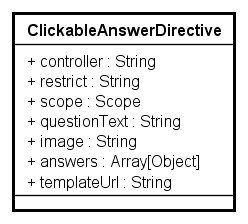
\includegraphics[scale=0.5,keepaspectratio]{UML/Classi/Front-End/QuizziPedia_Front-end_Templates_ClickableAnswerTemplate.png}
		\caption{QuizziPedia::Front-End::ModelViews::HomeModelView}
	\end{figure} \FloatBarrier
	
	\begin{itemize}
		\item \textbf{Descrizione}: ;
		\item \textbf{Utilizzo}: ;
		\item \textbf{Relazioni con altre classi}: 
		\begin{itemize}
			\item \textit{IN} \texttt{View}: ; 
			\item \textit{IN} \texttt{Controller}: ;
		\end{itemize}
		\item \textbf{Attributi}: 
		\begin{itemize}
			\item ;
		\end{itemize}
		\item \textbf{Metodi}: 
		\begin{itemize}
			\item ;
		\end{itemize}
	\end{itemize}	
